\pdfvariable minorversion 7\relax
\documentclass[aspectratio=169]{rosenpass-beamer}
\usepackage[english]{babel}
\usepackage{booktabs}

\usepackage{tikzsymbols}
\usepackage{multirow}
\usepackage{stmaryrd}
\usepackage[dvipsnames]{xcolor}
\usepackage{ulem}

\newcommand*{\heading}[1]{%
  {
    \hspace*{-0.5cm}#1
    \vspace{1.0em}
  }
}

%TODO Short title for the headline?
\title{The real-world security of Rosenpass \& WireGuard}
% \subtitle{\texorpdfstring{\vspace{0.2em}}{}}
\author{Karolin Varner \\ \footnotesize with support from Benjamin Lipp, Lisa Schmidt, and Marei Peischl}
\institute{\url{https://rosenpass.eu}}

\conference{Bergische Universität Wuppertal}
\date{2025-07-16}

\usepackage{biblatex}
\addbibresource{sources.bib}

\graphicspath{{}{graphics/}}

\usepackage{transparent}
\usepackage{colortbl}
\usepackage{pdfpc}

% Syntaxerweiterung \SetNextBackground{Bild} oder image= option bei frame

% \partnerlogo{%
% 	\includegraphics[height=2\baselineskip]{MPI-SP}%
% 	\includegraphics[height=2\baselineskip]{dlr}%
% }

% \ExplSyntaxOn
% \tl_gset:Nn \g__ptxcd_interlude_prefix_tl  {artsy-slide-backgrounds-smaller-hd/artsy-mild-bg-2}
% \int_gset:Nn \g__ptxcd_interlude_page_int {-1}
% \ExplSyntaxOff

\begin{document}

\maketitle

\section{Section: Prelude}

\section{Section Intro}

\begin{frame}[c]{Der Plan}
  \small

  \begin{enumerate}
    \item \textbf{Wir stellen uns vor}
    \item \textbf{Safety \& Security: Kulturelle Aspekte}
    \item \textbf{Kryptografie und Avionik im Dialog}
    \item \textbf{Kryptoagilität erreichen}
  \end{enumerate}

	\vfill
	\qrcode[height=2.5cm]{https://github.com/rosenpass/slides/blob/main/2025-05-15-cast/slides.pdf}~Folien \hfill Full~Paper~\qrcode[height=2.5cm]{https://doi.org/10.1007/s13272-025-00806-5}

  \vfill
\end{frame}



\begin{frame}{Karolin Varner}
  \begin{columns}[fullwidth,c]
	\hspace*{.25\LeftSlideIndent}%
    \begin{column}{\dimexpr.7\linewidth-.25\LeftSlideIndent}
      \begin{itemize}
        \item Software-Entwicklerin \& Kryptografin
        \item 11 Jahre in der Industrie bei Startups und Konzernen
        \item Seit 2024 am Max-Planck-Institut für Sicherheit und Privatsphäre
        \item Initiatorin \& Leiterin des Rosenpass e.V.
        \item Arbeit an weiteren Projekten wie zum Beispiel der X-Wing~Chiffre
      \end{itemize}
    \end{column}%
    \begin{column}{.3\linewidth}
      \includegraphics[width=.92\linewidth,trim=200 0 100 0,clip]{graphics/karolin-varner.jpg}
    \end{column}
  \end{columns}
\end{frame}

\begin{frame}{Rosenpass e.V.}
  \begin{columns}[fullwidth,c]
  	\hspace*{.25\LeftSlideIndent}
    \begin{column}{.5\linewidth}
      \begin{itemize}
        \item 2023 gegründet zur Betreuung des gleichnamigen Projekts
        \vfill
        \item Absicherung von WireGuard gegen Attacken durch Quantencomputer mittels protocol-level Hybridisierung
        \item Institution für Translationsforschung in der Kryptografie
        \vfill
        \item Schnittstelle zwischen Forschung, Industrie und Gesellschaft
      \end{itemize}
      \bigskip
      \textbf{\url{rosenpass.eu}}
    \end{column}%
    \begin{column}{.5\linewidth}
%      \includegraphics[ width=.92\linewidth]{graphics/Illu-install.png}
		\makebox[\linewidth][c]{\includegraphics[width=1.3\linewidth,page=18]{hpke-slide-designs}\hskip1.5em}
    \end{column}%
  \end{columns}
\end{frame}

\interlude{What do we want?}

\begin{frame}[T]{}
  \centering

  What do we want?

  \only<2,3,4>{Data communication}
  \only<3,4>{\\Securely}
  \only<4>{\\Something something quantum}
\end{frame}

\begin{frame}[T]{}
  \begin{tabular}{lrr}
                         & QKD                                 & Computational Cryptography \\
    End to End Security  & No                                  & Yes                        \\
    Authentication       & Yes\footnote{Through Wegman-Carter} & Yes                        \\
    Commodity Hardware   & No                                  & Yes                        \\
    Data rates           & kilobits                            & Arbitrary                  \\
    Information-theoretic security\footnote{Everlasting Secrecy, the lack of algorithmic hardness assumptions}
      & (No)\footnote{Not with these data rates}
      & (Yes)\footnote{With a suitcase of hard drives containing keys} 
  \end{tabular}
\end{frame}

\begin{frame}[T]{How to secure the internet against quantum attacks}
  \centering
  With computational cryptography!
\end{frame}

\begin{frame}[T]{How to think about quantum key distribution?}
  \centering
  \includegraphics[height=\defaultframetextheight]{scientific/rosenpass-qkd.pdf}
  As a fail-over in case Post-Quantum Cryptography fails.
\end{frame}

\begin{frame}[T]{Data streams become gibberish}
  \centering
  PLACEHOLDER \\
  As a hardware-security measure.
\end{frame}

\begin{frame}[T]{}
  \centering

  What do we want?

  \only<2,3,4,5>{Data communication}
  \only<3,4,5>{\\on highly secure institutional networks}
  \only<4,5>{\\with hardware security measures\\especially QKD}
  \only<5>{\\interoperable with the internet}
\end{frame}

\ExplSyntaxOn
\int_gset:Nn \g__ptxcd_interlude_page_int {-1}
\ExplSyntaxOff

\interlude{How do we build it?}

\begin{frame}[T]{How about a key management system?}
  \begin{columns}[T,fullwidth]
    \hfill
    \begin{column}{.55\linewidth}
      \includegraphics[height=\defaultframetextheight,trim=65 0 65 0,clip]{comic/rosenpass-comic-rgm-2.png}
    \end{column}
    \begin{column}{.38\linewidth}
      \vspace{0.8em}
      \begin{itemize}
        \item Pretty expensive
        \item Pretty complicated
        \item Still requires IP-based networking
        \item One compromised node compromises the entire network
        \item Does not address how to create data channels
      \end{itemize}
    \end{column}
    \hfill
  \end{columns}
\end{frame}

\begin{frame}[T]{}
  \centering
  \includegraphics[height=\defaultframetextheight]{comic/rosenpass-comic-rgm-3.png}
  Key management systems evoke the image of a rube-goldberg machine.
\end{frame}

\begin{frame}[T]{}
  \centering
  PLACEHOLDER \\
  The internet is an architecture for \textbf{transport-agnostic} networking.
\end{frame}

\begin{frame}[T]{}
  \centering
  PLACEHOLDER \\
  Then QKD is just another transport technology, with extra security features.
\end{frame}

\ExplSyntaxOn
\int_gset:Nn \g__ptxcd_interlude_page_int {-1}
\ExplSyntaxOff

\interlude{The end!}

\begin{frame}[T]{}
  \begin{columns}[T,fullwidth]
    \hfill
    \begin{column}{.55\linewidth}
      \centering
      \includegraphics[height=\defaultframetextheight]{comic/rosenpass-comic-rgm-2.png}
      \\ Doing this securely means we need secure routing.
    \end{column}
    \begin{column}{.38\linewidth}
      \vspace{0.8em}
      With internet standard technologies:
      \begin{itemize}
        \item \textbf{SRv6} to fully control the routes packages take \\ …even if nodes not on the path are compromised.
        \item \textbf{HNCP} to learn the network topology \\ …and to automatically deploy networks in the first place.
      \end{itemize}
    \end{column}
    \hfill
  \end{columns}
\end{frame}

\begin{frame}[T]{}
  \centering
  \includegraphics[height=\defaultframetextheight]{comic/rosenpass-comic-rgm-2.png}
  \\ And we need end-to-end hybrid computational security.
  \\ For instance using Rosenpass for post-quantum security and WireGuard for classical security.
\end{frame}

\begin{frame}[T]{}
  \centering
  \includegraphics[height=\defaultframetextheight]{comic/rosenpass-comic-rgm-2.png}
  \\ Ingress to egress security can substitute for end to end security in corporate environments
  \\ …so the technology does not have to be installed on every old windows laptop.
\end{frame}

\begin{frame}[T]{}
  \begin{columns}[T,fullwidth]
    \hfill
    \begin{column}{.55\linewidth}
      \centering
      \includegraphics[height=\defaultframetextheight]{comic/rosenpass-comic-rgm-2.png}
      \\ Comparing the architectures
    \end{column}
    \begin{column}{.38\linewidth}
      \vspace{0.8em}
      With internet standard technologies:
      \begin{itemize}
        \item QKD becomes just another transport
        \item KMS replaced with HNCP (observability) and SRv6 (secure routing)
        \item Management application package ties this into a neat bundle
      \end{itemize}
      Additional features:
      \begin{itemize}
        \item Interoperability with the normal internet
        \item Hardware security measures other than QKD supported
        \item Automatic network deployment through HNCP
      \end{itemize}
    \end{column}
    \hfill
  \end{columns}
\end{frame}

\ExplSyntaxOn
\int_gset:Nn \g__ptxcd_interlude_page_int {-1}
\ExplSyntaxOff

\interlude{This is in fact a Key Management System}

\begin{frame}[T]{}
  \centering
  \includegraphics[height=\defaultframetextheight]{comic/rosenpass-comic-rgm-2.png}
  \\ Keys sent on a secured path, gain the security properties of the secured path.
  \\ So we can implement a KMS, if we really want to, by exposing an API that chooses a random key, then transmits it.
\end{frame}

\begin{frame}[T]{}
  \centering
  \includegraphics[height=\defaultframetextheight]{comic/rosenpass-comic-rgm-2.png}
  \\ \textbf{Information theoretic security:} supported if the transports do support it.
\end{frame}

\begin{frame}[T]{}
  \centering
  \includegraphics[height=\defaultframetextheight]{comic/rosenpass-comic-rgm-2.png}
  \\ Quantum repeaters: Just a special type of transport, no distinction for the network.
\end{frame}

\interlude{What about a proper QKD-enabled internet?}

\begin{frame}[T]{}
  \centering
  \includegraphics[height=\defaultframetextheight]{comic/rosenpass-comic-rgm-2.png}
  \\ \textbf{Do not reinvent the wheel}, use established routing protocols:
  \\ Build an extension to IPv6, that can transmit QKD keys alongside packages.
\end{frame}

\begin{frame}[T]{}
  \centering
  \includegraphics[height=\defaultframetextheight]{comic/rosenpass-comic-rgm-2.png}
  We are collaborating with Quantum Optics Jena to realize this
\end{frame}

\ExplSyntaxOn
\int_gset:Nn \g__ptxcd_interlude_page_int {-1}
\ExplSyntaxOff

\interlude{Key takeaways}

\begin{frame}[T]{}
  \begin{columns}[T,fullwidth]
    \hfill
    \begin{column}{.55\linewidth}
      \centering
      \includegraphics[height=\defaultframetextheight]{comic/rosenpass-comic-rgm-2.png}
    \end{column}
    \begin{column}{.38\linewidth}
      \vspace{0.8em}
      Key takeaways:
      \begin{itemize}
        \item QKD is a hardware security measure, not a replacement for cryptography
        \item Key management systems are overcomplicated and not actually needed
        \item We can use or extend standard internet technologies, to build the quantum internet
      \end{itemize}
    \end{column}
    \hfill
  \end{columns}
\end{frame}



\end{document}
